\documentclass[DM,authoryear,toc]{lsstdoc}
% lsstdoc documentation: https://lsst-texmf.lsst.io/lsstdoc.html
\input{meta}

% Package imports go here.
\usepackage{graphicx}
\usepackage{url}
\usepackage{latexsym}
\usepackage{color}
\usepackage{enumitem}

% Local commands go here.

%If you want glossaries
%\input{aglossary.tex}
%\makeglossaries

\title{Detection Efficiencies for diaSources.}

% Optional subtitle
% \setDocSubtitle{A subtitle}

\author{%
Melissa Graham, 
Eric Bellm,
Leanne Guy,
and the Data Management System Science Team
}

\setDocRef{DMTN-231}
\setDocUpstreamLocation{\url{https://github.com/lsst-dm/dmtn-231}}

\date{\vcsDate}

% Optional: name of the document's curator
% \setDocCurator{The Curator of this Document}

\setDocAbstract{%
DRAFT. {\it Work in progress, see Section~\ref{sec:oq}}. This document describes how the Data Management System will determine and provide detection efficiencies for point-like {\tt diaSources} using artificial source injection. The scientific motivation and technical considerations are discussed.}

% Change history defined here.
% Order: oldest first.
% Fields: VERSION, DATE, DESCRIPTION, OWNER NAME.
% See LPM-51 for version number policy.
\setDocChangeRecord{%
  \addtohist{1}{YYYY-MM-DD}{Unreleased.}{Melissa Graham}
}


\begin{document}

% Create the title page.
\maketitle
% Frequently for a technote we do not want a title page  uncomment this to remove the title page and changelog.
% use \mkshorttitle to remove the extra pages

% ADD CONTENT HERE
% You can also use the \input command to include several content files.

% % % % % % % % % % % % % % % % % %
\section{Introduction} \label{sec:intro}

Any astrophysical question which asks, e.g., {\it "How often?"} or {\it "How many?"} about time-variable phenomena, such as population studies or occurrence rates, needs to know a survey's {\it detection efficiency}: the probability that a time-varying source is detected (or in other words, the fraction of all time-varying sources that are detected).

Detection efficiencies are required for many of the core science pillars of the LSST, such as transient phenomena, cosmology, and Solar System studies; injecting synthetic sources and reprocessing images is a common method for deriving detection efficiency (Appendix~\ref{sec:sci}).

Rubin Observatory documentation contains several requirements related to producing detection efficiencies for sources in difference images using synthetic source injection ({\tt diaSources}; Appendix~\ref{sec:docs}).
Leaving this to be a user-generated data product would be a moderate risk to LSST science (Appendix~\ref{sec:opts}).

This document describes how the Data Management (and/or the Rubin Data Production team in Operations) will make detection efficiencies available to users by:

\begin{enumerate}
\item injecting synthetic point-sources into a subset of images and reprocessing them with the Prompt and Data Release difference-image analysis pipelines;
\item ensuring the synthetic sources cover the range of parameters needed to determine detection efficiencies for transients and variables;
\item providing to users a catalog of injected sources, their simulated and measured properties, and whether they were detected; and
\item generating and serving a table of detection efficiencies.
\end{enumerate}

Readers should refer to the Data Products Definitions Document \citedsp{LSE-163} for more information about DIA, difference images, and {\tt diaSources}.
Detection efficiencies of extended difference-image sources (e.g., light echoes, trailed moving objects) are beyond the scope of this document.


% % % % % % % % % % % % % % % % % %
\clearpage
\section{Open Questions}\label{sec:oq}

\begin{enumerate}
\item \textbf{What is the available computational budget for reprocessing images?} Appendix B says ``the DMS computational system is sized to accommodate the (re)processing of all images with fake sources implanted (from KT)", but this comment is old (2019 or earlier) and should be reconfirmed. To go in Section~\ref{sec:tech}.
\item \textbf{How many injected sources are required to sufficiently characterize the detection efficiency?} Such as the number of ccds/night, number of sources/ccd, and especially, the number needed as a function of parameters $\vv{P}$: more fake sources will likely be needed for poor image quality, high local surface brightness, etc.
\end{enumerate}

For the latter, use existing detection efficiency papers from other surveys to evaluate how detection efficiency typically varies with image quality (and other parameters $\vv{P}$), in order to estimate how many injected sources will be needed.
Could use the OpSim (baseline) to evaluate how many images LSST will have with a given IQ to evaluate whether a random selection of visits and ccds would be sufficient, or if they must be chosen specifically. 


% % % % % % % % % % % % % % % % % %
\section{Technical Considerations}\label{sec:tech}

TBD.



% % % % % % % % % % % % % % % % % %
\clearpage
\section{Detection Efficiency Data Products}\label{sec:dedp}

{\bf Detection:} sources in difference images with a signal-to-noise ratio $SNR > {transSNR} = 5$ are considered {\it detected} and become a {\tt diaSource}\citedsp{LPM-17}.
 
{\bf Detection Efficiency:} The probability that a true variable or transient astrophysical source with a given difference-image flux is detected and becomes a {\tt diaSource}.
(In other words, the fraction of all true variable or transient astrophysical sources with a given difference-image flux that are detected and become a {\tt diaSource}).

The detection efficiency data products will include: 

\begin{itemize}
\item a catalog of metadata for injected sources (see below)
\item catalogs similar to {\tt diaSource} and {\tt diaForcedSource} that contain only recovered injected sources
\item a table of derived detection efficiencies ($\eta(m,\vv{P})$, see Section~\ref{ssec:dedp_pars}
\end{itemize}

The catalog of metadata for injected sources will include:

\begin{itemize}
\item identifiers for the direct and template images
\item pixel and sky coordinates
\item flux or magnitude (for direct and template)
\item the parameters described in Section~\ref{ssec:dedp_pars}
\end{itemize}

The injected source metadata will include sufficient information to recreate the exact PSF that was injected, so that images with injected sources do not need to be persisted.


\subsection{Methods for Generating Detection Efficiencies}\label{ssec:dedp_gen}

Detection efficiencies are typically generated by injecting synthetic sources into images -- into both the template and direct images or just the direct image, to simulate stars or transients respectively -- using a point-spread function shape similar to real astrophysical sources, and then reprocessing the images with the survey's difference image analysis pipeline and measuring the fraction detected in the difference image.

For the LSST, detection efficiencies will be derived for both the Prompt and Data Release (DR) difference image analysis (DIA) pipelines, because they are a bit different\footnote{Differences between the Prompt and DR DIA pipelines are imposed by the Prompt pipeline's 60 second limit.}.

For both the Prompt and DR pipelines, it is likely that the {\it full} pipeline need not be run -- sources could probably just be injected into the processed visit image (i.e., all prior stages can be skipped), then difference images generated, and then source detection and measurement run on the difference image (i.e., source association can be skipped).

For the Prompt pipeline, sources will \emph{not} be injected into new images as a part of Prompt processing.
Instead, the Prompt pipeline will be rerun on a subset of the night's images with sources injected.
The detection efficiency data products for the Prompt pipeline will thus be updated within the 24 hour timescale (similar to the Prompt Products Database), not on the 60 second timescale.

For the DR pipeline, the detection efficiency data products will be released on an annual basis along with the other DR data products.

For both the Prompt and DR detection efficiencies, the same parameters for synthetic sources (Section~\ref{ssec:dedp_pars}) will be used, and the locations of detected {\tt diaSources} will be avoided. 



\subsection{Parameters for Characterizing Detection Efficiencies}\label{ssec:dedp_pars}

The detection efficiency can be characterized as $\eta(m)$, where $m$ is the apparent magnitude of the time-changing component with respect to the template image, and $\eta$ is a value between $0$ and $1$ that represents the probability that the source would be detected in the difference image.
As described in Appendix~\ref{sec:sci}, $\eta$ depends on more than just $m$, and is a function several other parameters ($\vv{P}$), such as those listed in Table \ref{tab:eta_pars}.

An accurate measure of $\eta(m,\vv{P})$ for every pixel of every difference image is technologically unfeasible.
Instead, an analytic model for $\eta(m,\vv{P})$ can be built, so long as the synthetic sources cover the full range of $m$ and $\vv{P}$, and a sufficient number of synthetic sources are injected to measure how $\eta$ varies with $m$ and $\vv{P}$.

\textbf{The final list of parameters, the fraction of CCDs that will need to be reprocessed, and the number of injected sources per CCD all remain To Be Determined (Section~\ref{sec:oq}).}

\begin{table}[h]
\begin{center}
\begin{footnotesize}
\caption[]{A description of the potential image and source parameters ($\vv{P}$) that can affect the detection efficiency ($\eta(m)$) of point sources in a difference image (per filter).}
\label{tab:eta_pars}
\setlength{\extrarowheight}{5pt}
\begin{tabular}{|p{3.1cm}|p{12cm}|}
\hline
{\bf Parameter} & {\bf Description} \\
\hline
Surface Brightness & Typically, $\eta$ decreases for objects embedded in brighter host galaxies. \\
\hline
Point-Source Brightness & For stars, $\eta$ will depend on its magnitude in the template image. \\
\hline
Static-Source Offset & Sometimes, $\eta$ decreases for objects that are near (i.e., overlap the point-spread function of) static sources (e.g., AGN, galaxy cores, especially if cuspy in profile). \\
\hline
Field Crowdedness & $\eta$ for stars will likely depend on field crowdedness (e.g., stars per square arcmin). \\
\hline
CCD Location & With some instruments, $\eta$ decreases near the CCD edges due to distortion. \\
\hline
Image FWHM & The value of $\eta$ can decrease for extreme FWHM differences from the template (i.e., very good or very poor seeing). \\
\hline
Image Airmass & LSST images will experience differential chromatic refraction which affects image subtraction \citedsp{DMTN-037}, and thus potentially also $\eta$. \\
\hline
Sky Brightness & Typically, $\eta$ decreases when the sky background is bright or has a strong gradient (e.g., during twilight, near the moon). \\
\hline
Sky Cloud Cover & Extinction will affect $\eta$ by degrading the image magnitude limit. \\
\hline
\end{tabular}
\end{footnotesize}
\end{center}
\end{table}


\subsubsection{Parameters that do not need to be considered.}\label{sssec:dedp_pars_no}

As described in Appendix~\ref{sec:sci}, for $\eta(m,\vv{P})$ the synthetic sources do {\it not} need to accurately represent astrophysical transient types in terms of their colors, redshifts, host offsets, durations, light curves, etc.
That aspect of the analysis is best left to the user to handle for their particular type of object.

A specific example of how users might apply $\eta(m,\vv{P})$ in their analysis is provided in Appendix~\ref{ssec:sci_cfht}.
Generally, it would involve simulating a set of light curves for the object type of interest (e.g., normal $0.1<z<0.5$ Type Ia supernovae), and then using the detection efficiency table to evaluate the fraction that would be ``identified" in a given time-frame (where ``identified" might additional specific criteria in addition to detection as a {\tt diaSource}, such as a reliable photometric classification).
This is typically done as part of an MC analysis in order to marginalize over intrinsic distributions of, e.g., the brightness or host offsets of the object type of interest.


\appendix
% Include all the relevant bib files.
% https://lsst-texmf.lsst.io/lsstdoc.html#bibliographies
\section{References} \label{sec:bib}
\renewcommand{\refname}{} % Suppress default Bibliography section
\bibliography{local,lsst,lsst-dm,refs_ads,refs,books}

% Make sure lsst-texmf/bin/generateAcronyms.py is in your path
\section{Acronyms} \label{sec:acronyms}
\input{acronyms.tex}
% If you want glossary uncomment below -- comment out the two lines above
%\printglossaries


\clearpage
\section{Scientific Examples}\label{sec:sci}

Detection efficiencies are required for many of the core science pillars of the LSST, as described below.
Many other surveys use populations of synthetic sources injected into the data in order to characterize the detection efficiency, as described in the examples provided in \ref{ssec:sci_trans}.

In consideration of the scientific motivation for detection efficiencies, and what has worked for other surveys, two points are clear.

\begin{enumerate}

\item The population of synthetic sources injected in order to characterize the detection efficiency should have similar distributions as real astrophysical phenomena in terms of brightness and location (e.g., proximity to static-sky sources, field crowdedness, surface brightness), and the subset of images used should sample the distributions of, e.g., image quality (seeing), sky brightness, and airmass. 

\item The simulated fakes do not need to accurately represent astrophysical transient types, colors, redshifts, durations, light curves, etc., or be planted in sequential images in a correlated way to represent real light curves.
That aspect of the analysis is best left to the user to handle during the MC simulation stage for their particular type of object.

\end{enumerate}

% % % % % % % % % % % % % % % %
\subsection{Transients}\label{ssec:sci_trans}

Transient events such as stellar explosions (supernovae, kilonovae) and tidal disruption events (TDEs; stars destroyed by close passage to a supermassive black hole) occur once and do not repeat.
Since most transient progenitors are stars, they are most often found in high surface brightness environments (i.e., galaxies; their spatial distribution ``follows the light") and require difference imaging in order to be discovered, and thus detection efficiencies in order to characterize their occurrence rates.

For example, transient occurrence rates as a function of environment can constrain their progenitor star characteristics, which requires that detection biases be well known, as does understanding selection biases in transient samples (e.g., when using Type Ia supernova as cosmological standard candles). 

The four surveys mentioned below have either inserted fakes into all of their live images (SDSS-II and DES) or into a representative set of images at a later time (CFHT and PTF), to ensure that detection efficiencies can be determined for the full range of image parameters.
In all cases, the fakes were simulated with parameter distributions (e.g., brightness, location) that roughly mimic the real astrophysical objects of interest for each particular survey (mostly supernovae, for the above examples).
Typically, the MC method was then used to simulate light curves for the transient of interest, and then the derived detection efficiencies were applied.

The take-away message is that, for Rubin Observatory to best serve a broad section of the transient community, the simulated population of fake sources need only be representative of true astrophysical sources in a bulk sense, in terms of their brightness and location (i.e., plant more faint sources than bright, and more in high surface-brightness areas than isolated regions).
The simulated fakes do not need to accurately represent astrophysical transient types, colors, redshifts, durations, light curves, etc., or be planted in sequential images in a correlated way to represent real light curves.
That aspect of the analysis is best left to the user to handle during the MC simulation stage for their particular transient type. 

\subsubsection{Sloan Digital Sky Survey II (SDSS-II)}

In order to calculate the occurrence rates of Type Ia supernovae (SNe\,Ia) from the SDSS-II, \cite{2008AJ....135..348S} generated a realistic sample of SNe\,Ia and injected fake point sources into the images as part of the live data processing pipeline to discover SNe\,Ia.
Additional simulations to evaluate on how often the fakes were recovered by the end-to-end SN\,Ia discovery pipeline were then required to evaluate how assumptions about the simulated population (e.g., the distribution of light curve stretches) contributed to the final uncertainty in the derived rates \citep{2008ApJ...682..262D}.
The final form of their derived detection efficiency for SNe\,Ia was $\epsilon(z) = (0.78 \pm 0.01) + (-0.13 \pm 0.14)z$, within which is captured assumptions about the true relative fraction of each SN\,Ia subtype, such as the under/over-luminous 91bg/91T-likes \citep{2008ApJ...682..262D}.
The detection efficiency, $\epsilon$, contributed to the final volumetric rate, $r_V = N / \widetilde{VT\epsilon}$, where $N$ is the number of SNe\,Ia detected, and $\widetilde{VT\epsilon}$ is the product of the effective survey volume, time, and detection efficiency.

\subsubsection{Dark Energy Survey (DES)}

In order to determine the SN\,Ia detection efficiency as a function of redshift, the DES team used a method very similar to SDSS-II: fake sources were injected into their live data, which was run through their real-time {\tt DiffImg} pipeline used to detect transients \cite{2015AJ....150..172K}.
This process also started by simulating a realistic sample of SNe\,Ia, with parameters such as light curve stretch, host offset, and subtype drawn from established underlying distributions, and then used a Monte Carlo simulation of many more SN light curves, combined with the detection efficiencies for their fakes, to determine the SN\,Ia detection efficiency as a function of redshift.
% The DES real/bogus algorithm an pipeline are described by Goldstein et al. 2015:
% http://adsabs.harvard.edu/abs/2015AJ....150...82G

\subsubsection{A Canada-France-Hawaii Telescope (CFHT) Cluster Survey}\label{ssec:sci_cfht}

In order to calculate the occurrence rate of SNe\,Ia in galaxy clusters for a CFHT imaging survey, \cite{2012ApJ...746..163S} performed DIA to detect SNe in real time, but the fake injection was done separately.
Simulated point sources were implanted into a representative subset of their images, and detection efficiencies calculated as a function of the relevant parameters for this survey: apparent magnitude, image quality, and focal plane location (because because the survey used single pointings with only small dithers).
Their expression for the rate of Type Ia supernovae per unit stellar mass is $R_{\rm Ia} = (N_{\rm Ia} / C_{\rm spec}) / ( \sum_{j=1}^{j=N_{\rm img}} \Delta t_j Mj )$, where $N_{\rm Ia}$ is the number of SNe\,Ia discovered in the survey, $C_{\rm spec}$ is the spectroscopic confirmation rate (determined separately), the denominator's sum is over all images of the survey, $M_j$ is the total stellar mass within the image, and $\Delta t_j$ is the control time for SNe\,Ia of that image.
The control time is expressed as $\Delta t = \int_{t_1}^{t_2} \eta(m(t)) dt$, where $m(t)$ is a SN\,Ia light curve, $\eta$ is the detection efficiency, and the integration limits are the survey's temporal boundaries.

The Monte Carlo method was then used to calculate $R_{\rm Ia}$ for the survey many times while sampling over a realistic distribution of SN\,Ia light curve properties for $m(t)$ and the errors in $N_{\rm Ia}$, $M_j$, and $eta$.
During this MC, an {\it effective} detection efficiency was used, which accounts for the possibility that the simulated SN\,Ia was detected in the previous two images: $\eta = \eta_j - \eta_j \eta_{(j-1)} - \eta_j \eta_{(j-2)} - \eta_j \eta_{(j-1)} \eta_{(j-2)}$ (as was appropriate for this surveys monthly cadence).
The final result was quoted as the median of the MC rates with $1\sigma$ errors. A similar methodology was applied to this survey's cluster SNe\,II in \cite{2012ApJ...753...68G}.

\subsubsection{Palomar Transient Factory (PTF)}

The PTF covered $8000$ square degrees with a three-to-five day cadence and generated over $1$ $\rm PB$ of data.
As detailed by \cite{2017ApJS..230....4F}, inserting fake sources into all of these images was both impractical and unnecessary.
Instead, they chose a single representative {\it field} and planted fake sources in all images of that field.
The fakes were given a uniform distribution in apparent magnitude, distributed in each image such that most of them are located within a galaxy, and then the PTF detection efficiencies were determined as a function of the apparent magnitude, the local surface brightness, and image parameters such as FWHM, airmass, moon illumination fraction, and sky background.
These detection efficiencies were used to derive the volumetric rate of normal SNe\,Ia \citep{2019MNRAS.tmp..772F}, of Ca-rich transients by \cite{2018ApJ...858...50F}, and of tidal disruption events (TDEs) by \cite{2018ApJS..238...15H}.
However, note that some rates analyses for TDEs have used aperture photometry and not difference imaging, and thus did not need fake injection for difference-image detection efficiencies (e.g., \cite{2016MNRAS.455.2918H}).

% Frohmaier uses stars from the field, not a simulated PSF: "clone-stamping".
% Frohmaier 2019 details: r_v(z) = (1/V deltaT) sum_{i=1}^N (1+z_i) / epsilon_i
% r_v(z) = volumetric rate of SNeIa at redshift z
% V = volume
% delta T = survey time
% sum over the number of SNeIa in the final sample
% (1+z_i) = cosmological time dilation factor
% epsilon_i = "detection efficiencies of each object"
% but note that epsilon != eta, rather epsilon is built from eta
% a large sample of SNeIa with realistic intrinsic properties are simulated, planted in the data, and then recovered, and then a grid of recovery fractions as a function of SNIa intrinsic properties and redshift is created, and those are the epsilons assigned to detected SNeIa


% % % % % % % % % % % % % % % %
\subsection{Active Galactic Nuclei}\label{ssec:sci_agn}

Active Galactic Nuclei (AGN) are powered by a supermassive black hole in the center of a galaxy, surrounded by a gas disk.
Their energy output is non-thermal emission from X-ray through to mid-infrared, including emission lines in the optical spectrum, and many (or most) AGN exhibit optical variability.
As such, they appear as a variable point source in the cores of galaxies.
Many studies of AGN use aperture photometry on direct images, and not difference imaging, because it is desirable to have the {\it entire} flux of the AGN's point source, not just the flux in its variable component.

% The first to use variability to select AGN was Sarajedini et al. 2003; an two-epoch HST survey.
AGN samples have typically identified using spectroscopic emission lines, optical colors, or by looking for excesses of radio, X-ray, or mid-infrared emission, but selection by optical variability is also an option and in particular it may be better at including low-luminosity AGN, as described by \cite[e.g.,][]{2008A&A...488...73T,2010ApJ...723..737V}.
The detection method of \cite{2008A&A...488...73T} uses image subtraction for the initial detection of AGN candidates, mainly because difference imaging was already done to find supernovae in the survey.
Aperture photometry is then performed on the candidates, and a variability threshold applied to form their final sample for spectroscopic follow-up.
\cite{2010ApJ...723..737V} skip the difference imaging step and use aperture photometry and a statistical analysis true variability to identify AGN.
Neither use the injection of fake point sources to evaluate their detection efficiencies, and instead use objects with spectra and/or X-ray detections to estimate their completeness.
% De Cicco et al. 2015 is very similar to Trevese, done in the VST-SUDARE/VOICE survey for SNe.
However, using spectra or X-ray to characterize the sample selection function of AGN identified by optical variability might not be possible in the LSST era, when optical variability becomes a more efficient and prolific way to discover a AGN \cite[e.g.,][]{2014ApJ...782...37C}, generating significantly larger, lower-luminosity, and/or higher-redshift samples, for which spectroscopic confirmation is more difficult.

Furthermore, TDE and SNe also occur in the cores of galaxies \citep[e.g.,][]{2009A&A...507L..17P,2012ApJ...744L..19K}, causing contamination of the AGN samples, and quantifying the rate of missed transients in the cores of galaxies remains an open problem.

Considering the needs of the AGN, TDE, and SN communities suggests that a population of fake injected transients to characterize the difference-image detection efficiency of point sources in galaxy cores would be scientifically beneficial.



% % % % % % % % % % % % % % % %
\subsection{Variable Stars}\label{ssec:sci_varstar}

A star's luminosity might exhibit intrinsic variability (e.g., RR Lyrae, Cepheids) and/or extrinsic variability (e.g., eclipsing binaries, exoplanet transits, or microlensing events).
In uncrowded fields, using direct images and the total flux is preferable to difference-imaging analysis for scientific studies that aim to identify and characterize variable stars.
However, in crowded fields such as the Galactic plane, identifying variable stars in difference images can be much easier because the difference image is not as (or not at all) crowded, compared to the direct image.

For example, the census of variable stars in crowded fields by \cite{2016A&A...588A.128F} describes how difference imaging is used, although it does not appear that injecting fake sources or deriving detection efficiencies was needed for their analysis.

It also seems that difference-image detection efficiencies are not needed for microlensing studies, for which it is a common methodology to fit a PSF to every pixel of a difference image, concoct a "light curve", and then statistically assess whether it is consistent with the expected shape of a microlensing event \cite{2015ApJ...806..161L}\footnote{Although \cite{2015ApJ...806..161L} does mention that detection efficiencies would be used in a paper in preparation.}. 

Despite difference-image detection efficiencies not playing a role in past variable star studies, they might still be needed for LSST analyses.
For example, injecting new fake sources in crowded stellar fields might be useful for detection efficiencies for stars which are too faint to have a counterpart in the template, but whose variable component makes them detectable by LSST for a short while.
This would apply to e.g., M-dwarf flares (a common contaminant in searches for young SNe) and microlensing events.

Simulating variability of stars that {\it are} present in the template image is beyond the scope of this document.


% % % % % % % % % % % % % % % %
\subsection{Moving Objects}\label{ssec:sci_move}

All of the moving objects identified by LSST will first be detected as difference-image sources, and detection efficiencies would be useful for population studies.
In epochs of non-detection, being able to obtain the detection efficiency at a predicted location (i.e., as a function of local surface brightness and image qualities) would be a useful quantity for science goals related to moving object populations.
The probability of, e.g., a faint asteroid's chance alignment over bright galaxies is small, and so fake injected point sources in empty locations may be more useful for moving object science --- these would be needed to simulate very high-redshift transients, as well.

A consideration of whether the injection of trailed sources is scientifically useful is left for other work.



\clearpage
\section{Requirements Review}\label{sec:docs}

There are four requirements related to producing or serving detection efficiencies for transient {\tt DIASources} in difference images: OSS-REQ-0352\ossreq{0352}, OSS-REQ-0353\ossreq{0353}, DMS-REQ-0097\dmreq{0097}, and DMS-REQ-0009\dmreq{0009}.

Relatedly, the SRD specifies the definition for ``detection" as $SNR>5$, the OSS specifies that spuriousness (see Appendix~\ref{sec:rb}) characterization be done {\it ``by insertion and recovery of artificial sources"}, and the DMSR specifies that {\it software} for fake injection is a deliverable of the DMS (\S~\ref{ssec:docs_dmsr}).
The DPDD and LPM-151 also contain some discussion relevant to detection efficiencies.

Together, these specifications indicate that the use of artificial source injection to determine detection efficiencies for {\tt DIASources} would not be an expansion of scope for DM.

As a final note, the DMS computational system is sized to accommodate the (re)processing of all images with fake sources implanted {\bf (from KT)}.


% % % % % % % % % % % % % % % % 
\subsection{Science Requirements Document (SRD, LPM-17)}

The SRD \citedsp{LPM-17}, V5.2.4 (Jan 30 2018), does not contain any requirements related to detection efficiencies.

The SRD does describe how the Prompt pipeline should provide {\it ``the fast release of data on likely optical transients ... detected above {\tt transSNR} signal-to-noise ratio in difference images"}, where {\tt transSNR} = 5 (page 41).
This is pertinent to detection efficiencies because it defines that all sources with $SNR \geq 5$ in a difference image are considered ``detected".


% % % % % % % % % % % % % % % % 
\subsection{Observatory System Specifications (OSS, LSE-30)}\label{ssec:docs_oss}

The OSS \citedsp{LSE-30}, V19.1 (July 30 2021) contains four requirements related to characterizing the spuriousness (also known as the ``real/bogus" parameter), completeness, and purity of LSST sources detected in difference images using artificial injected sources. 
See Appendix~\ref{sec:rb} for a primer on spuriousness, completeness, and purity.

``Characterizing completeness" requires detection efficiencies, so these are effectively also requirements on producing detection efficiencies. 

\begin{itemize}

\item OSS-REQ-0351\ossreq{0351}, {\it Difference Source Spurious Probability Metric}, specifies that {\it ``the Observatory shall develop a metric to characterize the probability of each reported difference source being spurious"} (Section 3.1.5.2.1.7.5).
The discussion further clarifies that {\it ``the performance of this metric will be assessed by simulations, by insertion and recovery of artificial sources, and comparisons to ground truth where known"}.

\item OSS-REQ-0352\ossreq{0352}, {\it Difference Source Sample Completeness}, specifies that {\it ``for each visit, the Observatory shall estimate the detected difference source sample completeness and purity as a function of the spuriousness metric threshold cut"} (Section 3.1.5.2.1.7.6).
The discussion further clarifies that {\it ``this information will aid the end
users in selecting the spuriousness threshold appropriate for their particular science case"}.
However, as this requirement cannot be met without {\it difference source sample completeness}, it cannot be met with out detection efficiencies.

\item OSS-REQ-0353\ossreq{0353}, {\it Difference Source Spuriousness Threshold - Transients}, specifies that {\it ``there shall exist a spuriousness threshold {\tt T} for which the completeness and purity of selected difference sources are higher than {\tt transCompletenessMin} (90\%)\reqparam{transCompletenessMin} and {\tt transPurityMin} (95\%)\reqparam{transPurityMin}, respectively, at the SNR detection threshold {\tt transSampleSNR} (6)\reqparam{transSampleSNR}. This requirement is to be interpreted as an average over the entire survey"} (Section 3.1.5.2.1.7.7).
As for OSS-REQ-0351, the discussion further clarifies that {\it ``the performance of this metric will be assessed by simulations, by insertion and recovery of artificial sources, and comparisons to ground truth where known"}.
As for OSS-REQ-0352, since this requirement cannot be met without {\it difference source sample completeness}, it cannot be met with out detection efficiencies.

\item OSS-REQ-0354\ossreq{0354}, is similar to OSS-REQ-0353 but defines a threshold for moving objects.

\end{itemize}

% Regarding spuriousness, the discussion for OSS-REQ-0351 further describes that the {\it ``spuriousness metric be prior free to the extent possible. For example, while it may make use of information from the source and image characterization (e.g., comparison of source to PSF morphology), as well as the information on the Telescope and Camera system (e.g., ghost maps, defect maps, etc.), it will not use any information about the astrophysical neighborhood of the source, whether it has been previously observed or not, etc. The intent is to avoid introducing a bias against unusual sources or sources discovered in unusual environments"}.


% % % % % % % % % % % % % % % % 
\subsection{Data Management System Requirements (DMSR, LSE-61)}\label{ssec:docs_dmsr}

The DMSR \citedsp{LSE-61}, V9.0 (Feb 12 2021) contains a few statements relevant to detection efficiencies. 

\begin{itemize}

\item DMS-REQ-0097\dmreq{0097}, {\it "Level 1 Data Quality Report Definition"}, specifies that the Data Management System (DMS) {\it ``shall produce ... indicators of data quality that result from running the DMS pipelines, including ... detection efficiency for point sources vs. mag for each utilized filter"} (Section 1.3.14).
Although DMS-REQ-0097 is derived from OSS-REQ-0131, {\it ``Nightly Summary Products"}, and seems more intended to produce a nightly summary of the general performance of the observatory and the DMS, it is still a requirement to provide scientifically useful detection efficiencies that are the topic of this document. 

\item DMS-REQ-0009\dmreq{0009}, {\it ``Simulated Data"}, specifies that {\it ``the DMS shall provide the ability to inject artificial or simulated data into data products to assess the functional and temporal performance of the production processing software"} (Section 3.2.1), and detection efficiencies would be part of that performance assessment.
This requirement is derived in part from OSS requirements 0351, 0353, and 0354 discussed above.

\end{itemize}


% % % % % % % % % % % % % % % % 
\subsection{Data Products Definitions Document (DPDD, LSE-163)}\label{ssec:docs_dpdd}

The DPDD \citedsp{LSE-163}, V3.6 (Dec 17 2021) is not a requirements document but does have some information relevant to detection efficiencies.

Table 1 lists a single float is also reserved for ${SNR}$ in the DPDD's {\tt DIASource} table, defined as the {\it ``signal-to-noise ratio at which this source was detected in the difference image"}.

Table 1 also lists a single float is reserved in the {\tt DIASource} table for the spuriousness parameter.
The DPDD's definition and description of spuriousness match the OSS requirement (i.e., this is a direct flow-down of OSS-REQ-0351\ossreq{0351}).

The {\tt DIASource} catalog table has three other relevant parameters listed that might be scientifically useful for analyses involving detection efficiencies:
\begin{itemize}
\item {\tt psLnL [float]} -- {\it Natural log likelihood of the observed data given the point source model.} This represents the probability that a detected source is a point source; detection efficiencies would not apply to non-point sources.
\item {\tt fpBkgd [float]} $\rm nJy/asec^2$ -- {\it Estimated background at the position (centroid) of the object in the template image.} This will be useful to provide detection efficiencies in difference images as a function of the background at that location.
\item {\tt fpBkgdErr [float]} $\rm nJy/asec^2$ -- {\it Estimated uncertainty of {\tt fpBkgd}.} Useful in the same way as {\tt fpBkgd}. 
\end{itemize}


% % % % % % % % % % % % % % % % 
\subsection{Data Management Science Pipelines Design (LDM-151)}\label{ssec:docs_ldm151}

\citeds{LDM-151}, V4.3 (Nov 10 2020), details the scientific design and implementation of the requirements set by the SRD, OSS, and DMSR, and the generation of the data products described in the DPDD.

Section 3, {\it ``Alert Production"}, states that {\it ``In this document we do not address estimation of the selection function for alert generation through the injection of simulated sources. Such a process could be undertaken in batch mode as part of the DRP."}

However, \citeds{LDM-151} does make two relevant statements about the {\tt spuriousness} parameter which describe how the real-bogus algorithm will likely {\it ``be based on a trained random forest classifier ... conditioned on the image quality and airmass"} (Section 3.2.4) and that it  {\it ``may use machine learning on other measurements or pixels"} (Section 6.7.2).


%Section 3.2.4, {\it ``Difference Imaging"}, states that {\it ``The application of spuriousness algorithms, also known as 'real-bogus', may be applied at this time dependent on whether the number of false positives is less than 50\% of the detected sources. ... The default technique will be based on a trained random forest classifier. It is likely that the training of this classifier will need to be conditioned on the image quality and airmass of the observations."} 

% Section 6.7.2, {\it ``Algorithms"}, states that the {\tt spuriousness} measurement is a {\it ``per-source measure of likelihood the detection is junk (in a difference image)"} that {\it ``may use machine learning on other measurements or pixels"} and {\it ``may be augmented by spuriousness measures that aren't purely per-source"}. Figure 12, a matrix showing the algorithms applied to the different types of measurements (single visit, difference image, etc.) shows that a different implementation or algorithm for {\tt spuriousness} will be used for the Difference Image Measurement compared to the Single Visit, Multi-Coadd, Multi-Epoch, and Forced Measurements.

% Section 5.6.3, {\tt MakeSelectionMaps}, states that this calibration step {\it ``is responsible for producing multi-scale maps that describe LSST's depth and efficiency at detecting different classes of object. The details of what metrics will be mapped, the format and scale of the maps (e.g. hierarchical pixelizations vs. polygons), and the way the metrics will be computed are all unknown".} It also states that this must be extendable to Level 3, but that {\it ``the details of what DM will provide still needs to be clarified to the community"}, and notes that the reprocessing time for fake plants could be prohibitive. However, this referring to the depth and efficiency of detecting static-sky objects in the direct images or deep coadds, not transients/variables in the difference images.



\clearpage
\section{A Primer on Spuriousness (Real/Bogus)}\label{sec:rb}

The completeness, purity, and spuriousness of samples of detected sources are all related to detection efficiencies. 

When source detection is performed on a difference image, both true astrophysical sources and artifact sources can be detected with $SNR > {transSNR} = 5$ and become {\tt DIASources}.
Examples of artifacts include, e.g., sources caused by telescope hardware, or incompletely removed cosmic rays (despite the fact that cosmic rays are real astrophysical messengers). 

{\bf Spuriousness ($\mathcal{S}$):} a parameter, typically between $0$ and $1$, which represents the probability that a source is astrophysical (values closer to $1$) or artifact (values closer to $0$).

The spuriousness is sometimes also called the {\it real/bogus score}.
It is typically determined by machine learning on many sources that were pre-classified as astrophysical (real) or artifact (bogus), and usually considers factors like the shape of the point source in the difference image (e.g., symmetry, sharpness). 

{\bf Spuriousness Threshold ($\tau_{\mathcal{S}}$):} a lower limit on spuriousness, $\mathcal{S}$, which can be applied to {\tt DIASources} to separate the "real" from the "bogus", and to thereby obtain a subset of {\tt DIASources} with a lower fraction of artifacts. 

The following definitions describe the classification of detected {\tt DIASources}, which were either truly real (astrophysical source) or truly false (artifact), as real or bogus by an applied spuriousness threshold $\tau_{\mathcal{S}}$:

\begin{tabular}{rl}
True Positive ($\mathit{TP}$) & A detected astrophysical source that was classified as real. \\
False Positive ($\mathit{FP}$) & A detected artifact that was classified as real. \\
True Negative ($\mathit{TN}$) & A detected artifact that was classified as bogus. \\
False Negative ($\mathit{FN}$) & A detected astrophysical source that was classified as bogus. \\
\end{tabular}

{\bf Completeness ($\mathcal{C}$):} the fraction of all detected astrophysical sources which are classified as real. This is also called the true positive rate, $\mathit{TPR} = \frac{\mathit{TP}}{\mathit{TP}+\mathit{FN}}$.

{\bf Purity ($\mathcal{P}$):} the fraction of all detected sources that were classified as real which are astrophysical in nature: $\frac{\mathit{TP}}{\mathit{TP}+\mathit{FP}}$. This is also called the {\it precision} or the {\it positive predictive value} ($\mathit{PPV}$) of a survey. 

The false positive rate\footnote{Note that in some published literature the false positive rate is instead defined as the fraction of all detected artifacts that were classified as real, $\mathit{FPR} = \frac{\mathit{FP}}{\mathit{TN}+\mathit{FP}}$.} is the fraction of all detected sources that were classified as real but which are artifacts: $\mathit{FPR} = 1 - \mathit{PPV} = \frac{\mathit{FP}}{\mathit{TP}+\mathit{FP}}$.

The relationship between the completeness and purity of a sample of {\tt DIASources} classified as real can be traced out by varying $\tau_{\mathcal{S}}$.

In Figure \ref{fig:comp_pure} we show, as an example, the relationship between the false positive rate ($\mathit{FPR}$; purity) and the missed detection rate ($\mathit{MDR}$; completeness) for different types of source classification (i.e., real/bogus) algorithms from the Palomar Transient Factory \citep[PTF;][]{2013MNRAS.435.1047B}.
This relationship is formally known as the Receiver Operating Characteristic (ROC) curve when it is plotted as the true positive rate {\it vs.} the false positive rate for a given {\tt transSNR}.

\begin{figure}
\begin{center}
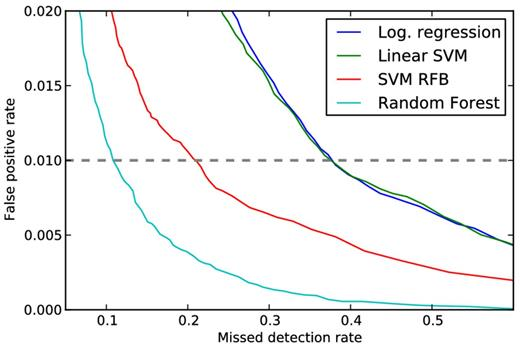
\includegraphics[width=8cm,trim={0cm 0cm 0cm 0cm}, clip]{figures/Brink_etal_2013_Fig3.jpg}
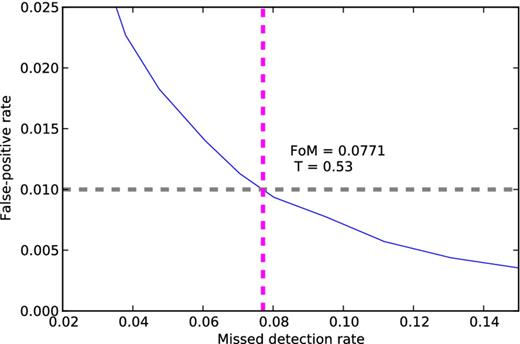
\includegraphics[width=8cm,trim={0cm 0cm 0cm 0cm}, clip]{figures/Brink_etal_2013_Fig7.jpg}
\caption{{\it Left:} An example of the relationship between the false positive rate ($\mathit{FPR}$; purity) {\it vs.} the missed detection rate ($\mathit{MDR}$; completeness) for different types of source classification (real/bogus) algorithms considered by the Palomar Transient Factory \citep{2013MNRAS.435.1047B}. {\it Right:} The relationship between $\mathit{FPR}$ and $\mathit{MDR}$ for the RB2 (real-bogus version 2) classifier (blue line) developed by the PTF and introduced in \cite{2013MNRAS.435.1047B}. Dashed lines show how $\mathit{FPR}=0.01$ is achieved with a spuriousness (real-bogus score value) threshold of $\tau=0.53$, which results in $\mathit{MDR}=0.077$. \label{fig:comp_pure}}
\end{center}
\end{figure}

{\bf Characterizing spuriousness} requires knowing which of the detected {\tt DIASources} are astrophysical (truly real) and which are artifacts (truly bogus).
Synthetic source injection is best for simulating astrophysical (real) sources because artifacts (bogus) can be a very diverse group; source injection cannot reveal which {\tt DIASources} in an image are artifacts.
Instead, characterizing spuriousness is achieved by building a training set of point sources that have been confirmed as astrophysical and artifact, using that training set for the spuriousness ($\mathcal{S}$; real/bogus) assignments by the machine learning algorithm.
Then, since ${transSNR}\propto m$, the ROC curve yields $\mathcal{C}(m,\tau_{\mathcal{S}})$ and $\mathcal{P}(m,\tau_{\mathcal{S}})$.


\clearpage
\section{Options Regarding Detection Efficiencies} \label{sec:opts}

Options are discussed in terms of the DM effort they require, the risks involved, and the science impact. 

The option in \ref{ssec:opts_3}, which requires a bit of extra DM effort to (1) ensure that the artificial sources synthesized and injected into images in order to characterize spuriousness cover the parameters needed for scientific analyses, $\vv{P}$ (Table \ref{tab:eta_pars}), and (2) to generate and provide a table of detection efficiencies, would moderately benefit LSST science.


% % % % % % % % % % % % % % % % 
\subsection{Do Nothing}\label{ssec:opts_no}

The science community would have access to only the software for synthetic source injection (DMS-REQ-0009, \ref{ssec:docs_dmsr}).

{\bf DM Effort -- None.}

{\bf Risk -- Major.}
Multiple user groups may then attempt wide-scale source injection and image re-processing, leading to redundant use of limited computational and human resources. 

{\bf Science Impact -- Negative.}
Lack of detection efficiencies might prohibit science investigations of transient phenomena, Solar System objects, and cosmology, or limit them to research groups able to put effort towards deriving detection efficiencies.


% % % % % % % % % % % % % % % % 
\subsection{Make Available the Artifical Sources Use for Spuriousness Characterization}\label{ssec:opts_1}

In this scenario, the science community would be given access to the tables of the synthetic sources that are injected into imaging data in order to meet the requirements to characterize the spuriousness parameter (OSS-REQ-0351, \ref{ssec:docs_oss}).

For example, this might take the form of a {\tt DIASource}-like catalog for the synthetic point sources (without the $SNR>5$ restriction), which users could bin by the $\vv{P}$ relevant to their science and generate $\eta(\vv{P})$.
Since the current OSS requirements are to characterize the relationship between spuriousness and sample completeness {\it only as a function of visit image qualities} for {\tt DIASources} with SNR$>$5 (\S~\ref{sec:docs}), this scenario does not guarantee that these artificial sources would be adequate for all science use-cases. 

{\bf DM Effort -- Minor.}
E.g., ingesting the synthetic source catalogs to qserv or the Butler.

{\bf Risk -- Moderate.}
It is unlikely that the synthetic sources injected for spuriousness characterization would adequately cover $\vv{P}$.
The DM effort to release the tables might not be worth it.

{\bf Science Impact -- Minor Benefit.}
Allowing users to build detection efficiency matrices from the same artificial sources as are used to characterize spuriousness might enable some scientific analyses.


% % % % % % % % % % % % % % % % 
\subsection{... And Optimize the Artificial Sources for Detection Efficiencies}\label{ssec:opts_2}

This scenario builds on the above, adding a bit of extra effort dedicated to ensuring the simulated sources that are injected and recovered in order to meet the requirements to characterize the spuriousness parameter cover the parameters needed for scientific analyses, $\vv{P}$, as listed in Table \ref{tab:eta_pars}.

{\bf DM Effort -- Minor.}
E.g., the extra time and effort to ensure the synthetic sources cover an adequate range of parameter space, $\vv{P}$ (plus the effort described above).

{\bf Risk -- Minor.}
With sufficient effort to make sure the synthetic sources are broadly useful, DM's efforts here would be worth it and be likely to benefit science.

{\bf Science Impact -- Moderate Benefit.}
Allowing users to build detection efficiency matrices from a scientifically-validated set of artificial sources would enable more scientific analyses.


% % % % % % % % % % % % % % % % 
\subsection{... And Generate and Provide Detection Efficiencies}\label{ssec:opts_3}

This scenario builds on the above, adding a bit of extra effort to generate and provide the detection efficiency matrix, $\eta(\vv{P})$.

{\bf DM Effort -- Moderate.}
E.g., the extra time and effort to generate the detection efficiency matrix and provide examples of how to use it (plus the efforts described above).

{\bf Risk -- Minor.}
It is very likely that this goal would be achievable and that this effort would be successful.

{\bf Science Impact -- Moderate Benefit}
Enables everyone in the science community to engage in the many different types of scientific analyses that require detection efficiencies.



% % % % % % % % % % % % % % % % 
\subsection{Further Considerations}\label{ssec:opts_plus}

{\bf Detection efficiencies should be generated on an annual timescale. -- }
The characterization of detection efficiencies is something that could (and should) only be done as part of the Data Release processing, on an annual timescale. 
Generally, the science investigations that require detection efficiencies would be done with the Data Release {\tt DIASource} catalog because they require a well-defined sample, and the Prompt {\tt DIASource} catalog will be constantly growing.
If needed, the DR-derived detection efficiencies could be used on the Prompt data products for the following year.

{\bf Separate Image Processing Required -- }
This may seem obvious, but: although some past surveys have injected synthetic sources into their raw data, allowing them to only process their images once and to conserve their total computational budget, this is not feasible for the LSST due to its wide variety of science use cases for the processed images and the high risk involved in contaminating the data.

In order to generate detection efficiencies, artificial sources do not need to be injected into {\it every} LSST image, only a representative sample.

{\bf Avoid Contamination -- }
Artificial sources should not be injected at random locations because it is important to sample regions with higher surface brightness and to avoid the locations of known {\tt DIAObjects}.
If 1000 artificial sources are assigned random locations and injected into a 3.2 Gp image, and we assume that image has 10000 (randomly-distributed) true sources in it, then the probability that none of the artificial sources are coincident with one of the true sources is $0.9968$.
However, over a full night of 1000 visits, the probability that none of the artificial sources ever landed on a true source in any image is $0.0437$, and it is most likely ($P=0.2218$) that 3 artificial sources would have interfered with true sources. 
% from scipy.stats import hypergeom
% import matplotlib.pyplot as plt
% [M,n,N] = [3200000000,10000,1000]
% rv = hypergeom(M,n,N)
% print( rv.pmf([0,1,2,3,4]) )
% [  9.96843454e-01   3.11521588e-03   4.86216368e-06   5.05362508e-09   3.93505558e-12]
% [M,n,N] = [3200000000000,10000000,1000000]
% rv = hypergeom(M,n,N)
% print( rv.pmf([0,1,2,3,4]) )
% [ 0.04367555  0.13880061  0.21497859  0.22180274  0.17274015]


\clearpage
\section{Artificial Source Injection Techniques}\label{sec:tech}

Describing the technique for artificial source injection that the LSST Science Pipelines will use is left for the Data Management Science Pipelines Design document, \citedsp{LDM-151}.

Typically, artificial sources are added to the direct image {\it before} that image enters the difference imaging pipeline, so that the detection efficiency captures the end-to-end pipeline efficiency for detecting difference-image sources.

{\bf Model PSF --}
A 2D model for the PSF is added to the direct image in order to simulate a new point source.
The shape of the PSF is derived from known trends with, e.g., the focal plane location or airmass (DCR), and the brighter/fatter effect.

{\bf Clone-Stamping --}
A nearby star is cut out and rescaled, and used as the simulated point source.
One of the main drawbacks of using clone-stamping with LSST images is that incorporating the brighter/fatter effect into the simulation requires either that a star which is both nearby and of a similar brightness be used or that a model component added to the clone star to appropriately change the shape for the simulated brightness.
Another drawback of clone-stamping is that very sparse/crowded fields might not have enough nearby/isolated point sources to use.

Techniques to simulate the variability of real astrophysical objects, such as stars with a time-variable component, are considered beyond the scope of this document.


\end{document}
